%========================
% Theme
%========================
\documentclass[8pt]{beamer}
\setbeamersize{text margin left=10mm,text margin right=10mm} 
\usetheme[progressbar=frametitle]{metropolis}
\usepackage{appendixnumberbeamer} % handles appendix slide numbering

%========================
% Packages: Icons and Tables
%========================
\usepackage{booktabs}        % professional tables
\usepackage[scale=1]{ccicons} % Creative Commons icons

%========================
% Packages: Plots and TikZ
%========================
\usepackage{pgfplots}
\usepgfplotslibrary{dateplot}

\usepackage{tikz}
\usetikzlibrary{positioning}

%========================
% Packages: Algorithms
%========================
\usepackage{algorithm}
\usepackage{algpseudocode}

%========================
% Packages: Math
%========================
\usepackage{amsmath,amsfonts,amsthm,amssymb}
\newtheorem{prop}{Proposition}

%========================
% Custom commands
%========================
\usepackage{xspace}
\newcommand{\themename}{\textbf{\textsc{metropolis}}\xspace}

%========================
% Custom footline
%========================
\setbeamertemplate{footline}
{%
  \leavevmode%
  \hbox{%
  \begin{beamercolorbox}[wd=.35\paperwidth,ht=2.5ex,dp=1.5ex,center]{author in head/foot}%
    \usebeamerfont{author in head/foot}\insertshortauthor
  \end{beamercolorbox}%
  \begin{beamercolorbox}[wd=.3\paperwidth,ht=2.5ex,dp=1ex,center]{title in head/foot}%
    \usebeamerfont{title in head/foot}\insertshorttitle
  \end{beamercolorbox}%
  \begin{beamercolorbox}[wd=.3\paperwidth,ht=2.5ex,dp=1ex,right]{date in head/foot}%
    \usebeamerfont{date in head/foot}\insertframenumber{} / \inserttotalframenumber
  \end{beamercolorbox}}%
  \vskip0pt%
}

%========================
% Remove default navigation symbols
%========================
\setbeamertemplate{navigation symbols}{}

\usepackage{pgf,pgfarrows,pgfnodes,pgfautomata,pgfheaps,pgfshade}
\usepackage{hyperref}
\usepackage{listings}
\usepackage{color}

\lstset{language=R,
    basicstyle=\small\ttfamily,
    stringstyle=\color{DarkGreen},
    otherkeywords={0,1,2,3,4,5,6,7,8,9},
    morekeywords={TRUE,FALSE},
    deletekeywords={data,frame,length,as,character},
    keywordstyle=\color{blue},
    commentstyle=\color{DarkGreen},
}

\usepackage{xcolor}

\lstset{
    language=Python,
    basicstyle=\ttfamily\small,
    keywordstyle=\color{blue},
    commentstyle=\color{gray},
    stringstyle=\color{red},
    breaklines=true,
    numbers=left,
    numberstyle=\tiny
}



%%%%%%%%%%%%%%%%%%%%%%%%%%%%%%%%%%%%%%%%%%%%%%%%%%%%%%%%%%%%%%%%%%%%
%%%%%%%%%%%%%%%%%%%%%%%%%%%%%%%%%%%%%%%%%%%%%%%%%%%%%%%%%%%%%%%%%%%%
% AQUI SE DEFINEN LAS IMAGENES PARA UTILIZAR DESPUES
%\pgfdeclareimage[interpolate=true, height=7cm,width=16cm]{halton-points}{halton-points}
%\pgfdeclareimage[interpolate=true, height=3cm, width =4cm]
%{serie-petroleo-reducido}{serie-petroleo-reducido}
%\pgfdeclareimage[interpolate=true, height=3cm, width =4cm]{rectangle-triangle}{rectangle-triangle}
%\pgfdeclareimage[interpolate=true, height=3cm, width =4cm]{any-angle}{any-angle}
%\pgfdeclareimage[interpolate=true, height=3cm, width =4cm]{Pythagoras}{Pythagoras}


\title{Chapter 1 - Random Number Generation}
\subtitle{The Inverse Transform Method}
\author{Prof. Alex Alvarez, Ali Raisolsadat}
\institute{School of Mathematical and Computational Sciences \\ University of Prince Edward Island}
\date{} % leave empty or add \today
%\title[Stat 4110]{Stat 4110 Statistical Simulation}
%\subtitle{}
%\author[University of Prince Edward Island]{School of Mathematical and Computational Sciences \\ University of Prince Edward Island}

%========================
% Begin document
%========================
\begin{document}

%-------------------
% Title frame
%-------------------
\maketitle

%-----------------------
% Slide 1: Inverse Transform Method
%-----------------------
\begin{frame}{Inverse Transform Method}
\textbf{General Quantile Function}: Let $F$ be a cumulative distribution function(c.d.f.). Then the inverse of $F$ is defined as 

\begin{equation*}
	F^{-1}(u)=\inf \left\{ x \in \mathbb{R} | F(x) \geq u \right\}
\end{equation*}

\pause

\textbf{Theorem}: Let $F: \mathbb{R} \rightarrow [0,1]$ be a c.d.f. and $F^{-1}$ its inverse. If $U \sim \text{uniform}[0,1]$ and we define $X=F^{-1}(U)$ then $X$ has c.d.f. $F$.

\vspace{2mm}
\pause

\textbf{Proof (Short Version)}: 
\begin{equation*}
	P(X\leq a)=P(F^{-1}(U) \leq a)=P(\inf \left\{ x \in \mathbb{R} | F(x) \geq U \right\} \leq a)
\end{equation*}

\vspace{2mm}

Since $\inf \left\{ x \in \mathbb{R} | F(x) \geq U \right\} \leq a$ holds if and only if $F(a)\geq U$ then

$P(X\leq a)=P(F(a) \geq U)=F(a)$ therefore X has c.d.f. F.

\vspace{2mm}

This result is very general (applicable to both continuous and discrete distributions).
\end{frame}

%-----------------------
% Slide 2: Inverse Transform Method
%-----------------------
\begin{frame}{Inverse Transform Method}
\textbf{Proof (Long Version)}: 

Let $U \sim \text{Uniform}(0,1)$ and define the generalized inverse of $F$ as
\begin{equation*}
F^{-1}(u) = \inf \{ x \in \mathbb{R} \mid F(x) \ge u \}
\end{equation*}

Let
\begin{equation*}
X = F^{-1}(U)
\end{equation*}

Then, for any $x \in \mathbb{R}$:
\begin{equation*}
P(X \le x) = P(F^{-1}(U) \le x)
\end{equation*}

By the definition of the generalized inverse:
\begin{equation*}
F^{-1}(U) \le x \iff U \le F(x)
\end{equation*}

Hence,
\begin{equation*}
P(X \le x) = P(U \le F(x)) = F(x)
\end{equation*}

This shows that $X$ has CDF $F$, regardless of whether $F$ is continuous or discrete.
\end{frame}

%-----------------------
% Slide 3: Algorithm for Explicit Inverse Transform Method
%-----------------------
\begin{frame}{Algorithm (Inverse Transform Method)}
\alert{Algorithm}
\begin{enumerate}
\item Generate $U \sim U[0,1]$ 
\item Define $X=F^{-1}(U)$
\item Return $X$

\end{enumerate}
\pause

{\bf Remarks:} 

\begin{itemize}

\item This method is more suited to continuous distributions, but it can also be applied to discrete distributions (See example 1.18 from the textbook).

\item An important limitation of the method is that can only be applied to one-dimensional probability distributions.

\end{itemize}
\end{frame}

%-----------------------
% Slide 4: Example function for inverse transform method
%-----------------------
\begin{frame}{Inverse Transform Example}
\textbf{Example}: Generate a sample of 5 random numbers from a continuous random variable with probability density function
\begin{equation*}
f(x)=\left\{ 
\begin{array}{ll} 
x^3/4  & \text { if } x \in [0,2]\\
 0 & \text{ otherwise} 
\end{array}
\right.
\end{equation*}

\pause

\textbf{Solution}: First we find the cumulative distribution function $F$.
\begin{equation*}
F(x)=\int_{-\infty}^x f(s)ds=
\left\{ 
\begin{array}{ll}
0 & \text{ if } x<0\\
x^4/16 & \text{ if } 0\leq x<2\\
1  & \text{ if } x \geq 2\\
\end{array}
\right.
\end{equation*}

From here we get $F^{-1}(x)=\sqrt[4]{16x}$
\end{frame}

%-----------------------
% Slide 5: Example function for inverse transform method
%-----------------------
\begin{frame}[fragile]{Inverse Transform Example}
\alert{Code}

\vspace{2mm}

\begin{columns}[T]
\begin{column}{0.4\textwidth}
\textbf{\textbf{R Code}}
\begin{lstlisting}
n <- 5
U <- runif(n, min=0, max=1)
X <- (16*U)^(1/4)
print(X)
\end{lstlisting}
\end{column}

\begin{column}{0.45\textwidth}
\textbf{Python Code}
\begin{lstlisting}[language=Python]
import numpy as np

n = 5
U = np.random.uniform(0, 1, n)
X = (16*U)**(1/4)
print(X)
\end{lstlisting}
\end{column}
\end{columns}
\end{frame}

%-----------------------
% Slide 6: Example (Exponential Distribution)
%-----------------------
\begin{frame}[fragile]{Inverse Transform Method: Exponential Distribution}
\textbf{Example (Exponential Distribution)}: Generate a sample of $n=100$ random numbers from the exponential distribution with parameter $\lambda=2$ using the inverse transform method. 

\vspace{2mm}

\pause

In general the density for the exponential distribution with parameter $\lambda$ is given by
\begin{equation*}
f(x)=\left\{ 
\begin{array}{ll}
\lambda e^{-\lambda x} & \text{ if } x \geq 0  \\
0 & \text { otherwise }
\end{array}
\right.
\end{equation*}

Then the cumulative distribution function is $F(x)=1-e^{-\lambda x}$ for $x\geq 0$.

The inverse function is $\displaystyle{F^{-1}(x)=-\frac{\ln(1-x)}{\lambda}}$
\end{frame}

%-----------------------
% Slide 7: Example (Exponential Distribution)
%-----------------------
\begin{frame}[fragile]{Inverse Transform Method: Exponential Distribution}
\alert{Code}

\vspace{2mm}

\begin{columns}[T]

\begin{column}{0.4\textwidth}
\textbf{R Code}
\begin{lstlisting}
n <- 100
lambda <- 2
U <- runif(n, min=0, max=1)
X <- -log(1-U)/lambda
print(X)
hist(X)
\end{lstlisting}
\end{column}

\begin{column}{0.45\textwidth}
\textbf{Python Code}
\begin{lstlisting}[language=Python]
import numpy as np
import matplotlib.pyplot as plt

n = 100
lambda_ = 2
U = np.random.uniform(0, 1, n)
X = -np.log(1-U)/lambda_
print(X)
plt.hist(X, bins=10)
plt.show()
\end{lstlisting}
\end{column}
\end{columns}

\pause

\textbf{Remark}: Of course, without the constraint of using the inverse transform method, we could use R's or Python's built-in exponential generator.
\end{frame}

%-----------------------
% Slide 8: Example (Exponential Distribution) plot
%-----------------------
\begin{frame}[fragile]{Envelope Rejection Sampling Example}
\begin{center}
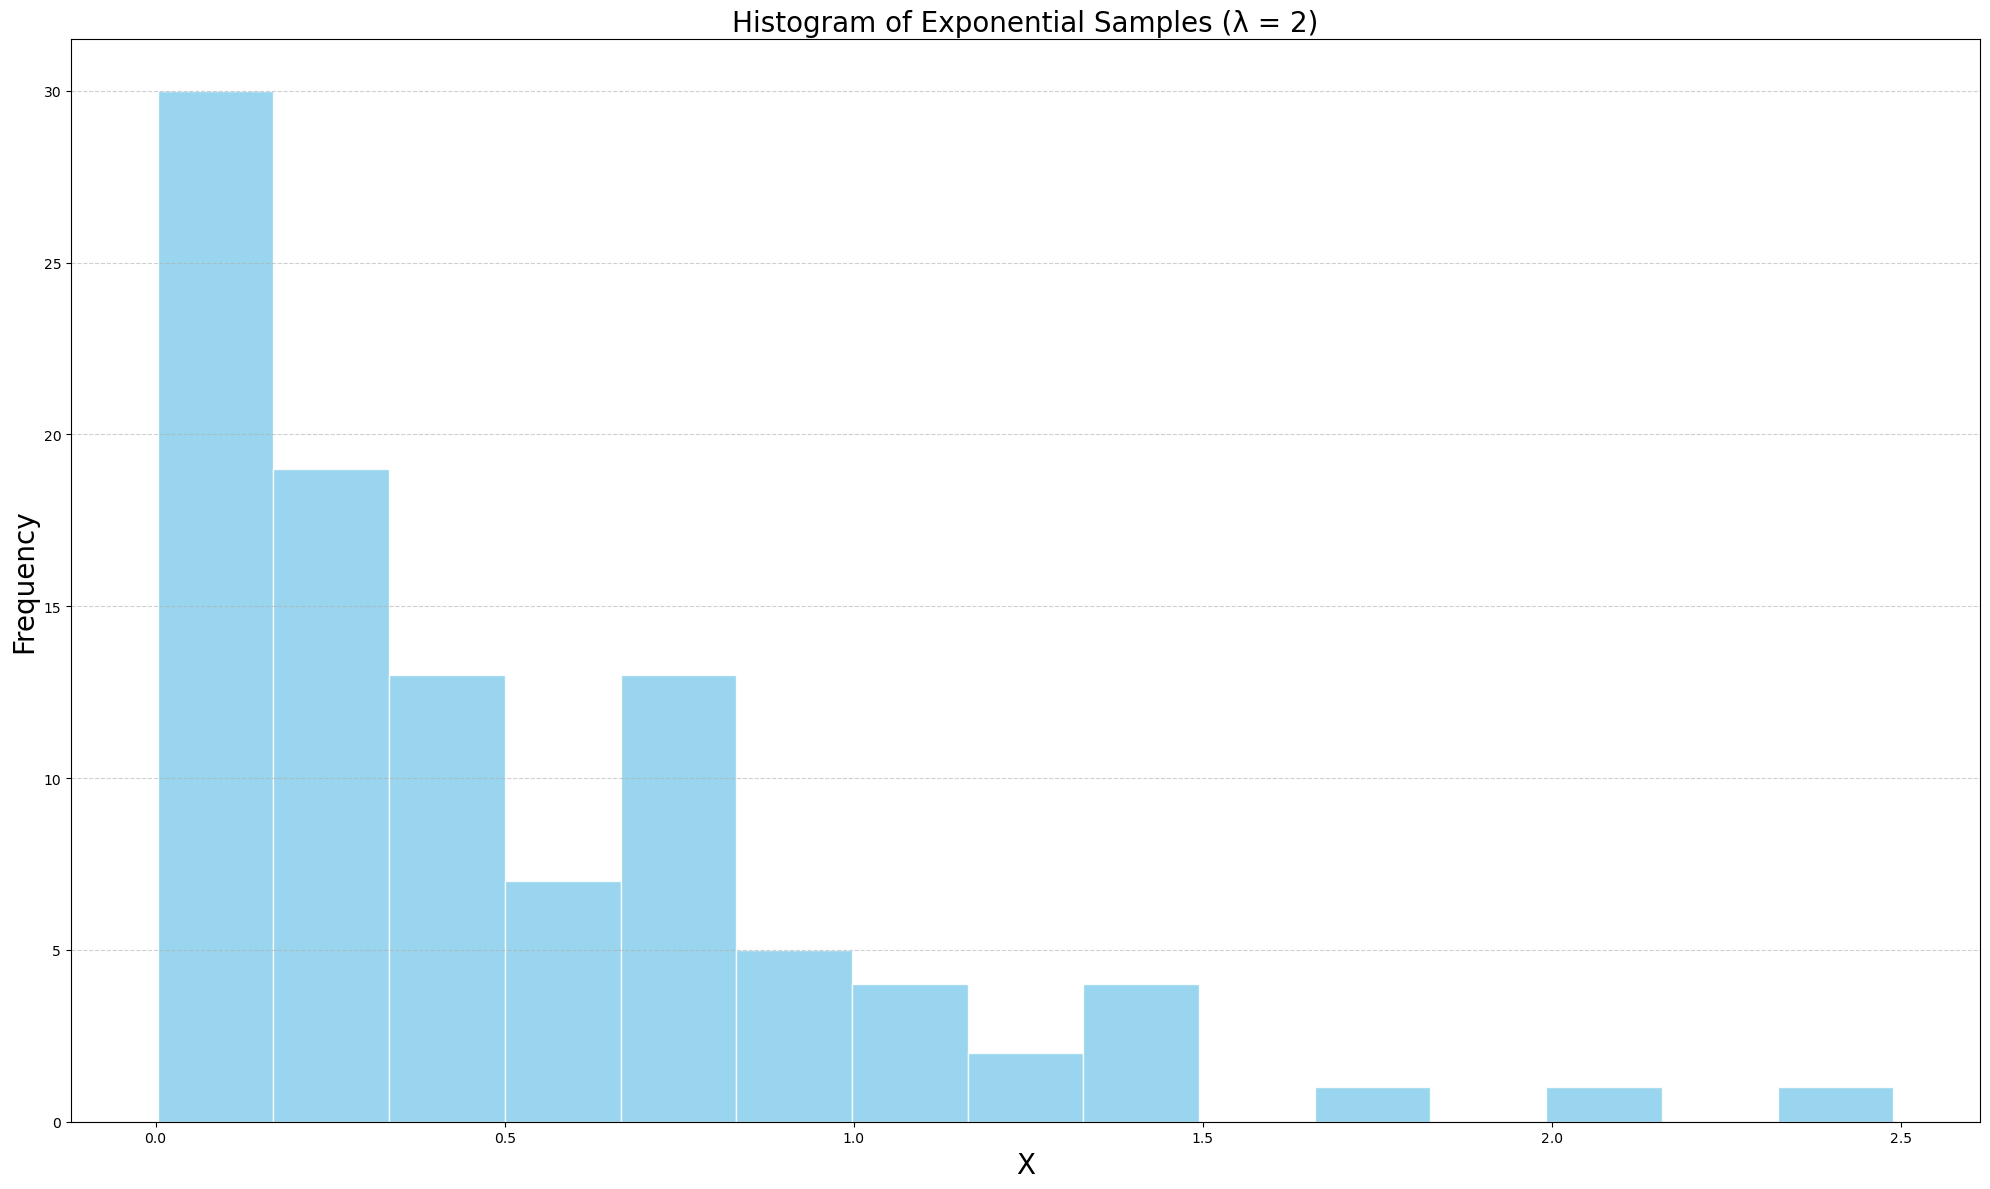
\includegraphics[width=\textwidth]{chapter1-part2-plot1.png}
\end{center}
\end{frame}


%-----------------------
% Slide 9: Summary
%-----------------------
\begin{frame}{Summary}
\begin{itemize}
	\item The inverse transform method is straightforward, efficient and very general.
	\item For the generation of continuous random variables, the inverse transform method is the method of choice in most cases, as long as $F^{-1}$ can be found explicitly.
	\item Unfortunately, some important distributions do not admit a closed-form solution for $F^{-1}$ (the normal distribution is an obvious example of this) therefore other methods would have to be applied in those cases.

\end{itemize}
\end{frame}

%-----------------------
% Slide 10: Homework
%-----------------------
\begin{frame}{Homework}
\begin{enumerate}
	\item Write down a computer program to generate a sample of 1000 random numbers from the probability distribution with density function 
\begin{equation*}
f(x) = \frac{3}{2} x^{-5/2}, \quad x \in [1, \infty), \quad 0 \text{ otherwise.}
\end{equation*}
	\item Find the explicit inverse of the CDF for the \textbf{Weibull distribution} $$F(x) = 1 - e^{-(x/\lambda)^k}, \ x \ge 0, \quad x \leq 0$$
	\item Find the explicit inverse of the CDF for the \textbf{Cauchy distribution} $$F(x) = \frac{1}{\pi} \arctan\left(\frac{x-x_0}{\gamma}\right) + \frac{1}{2}, \quad \gamma>0$$ 
	\item Find the explicit inverse of the CDF for the \textbf{Logistic distribution} $$F(x) = \frac{1}{1 + e^{-(x-\mu)/s}}, \quad s > 0$$ and plot both the PDF and CDF. What is the difference between this distribution and the \textbf{Normal distribution}?
\end{enumerate}
\end{frame}


\end{document}